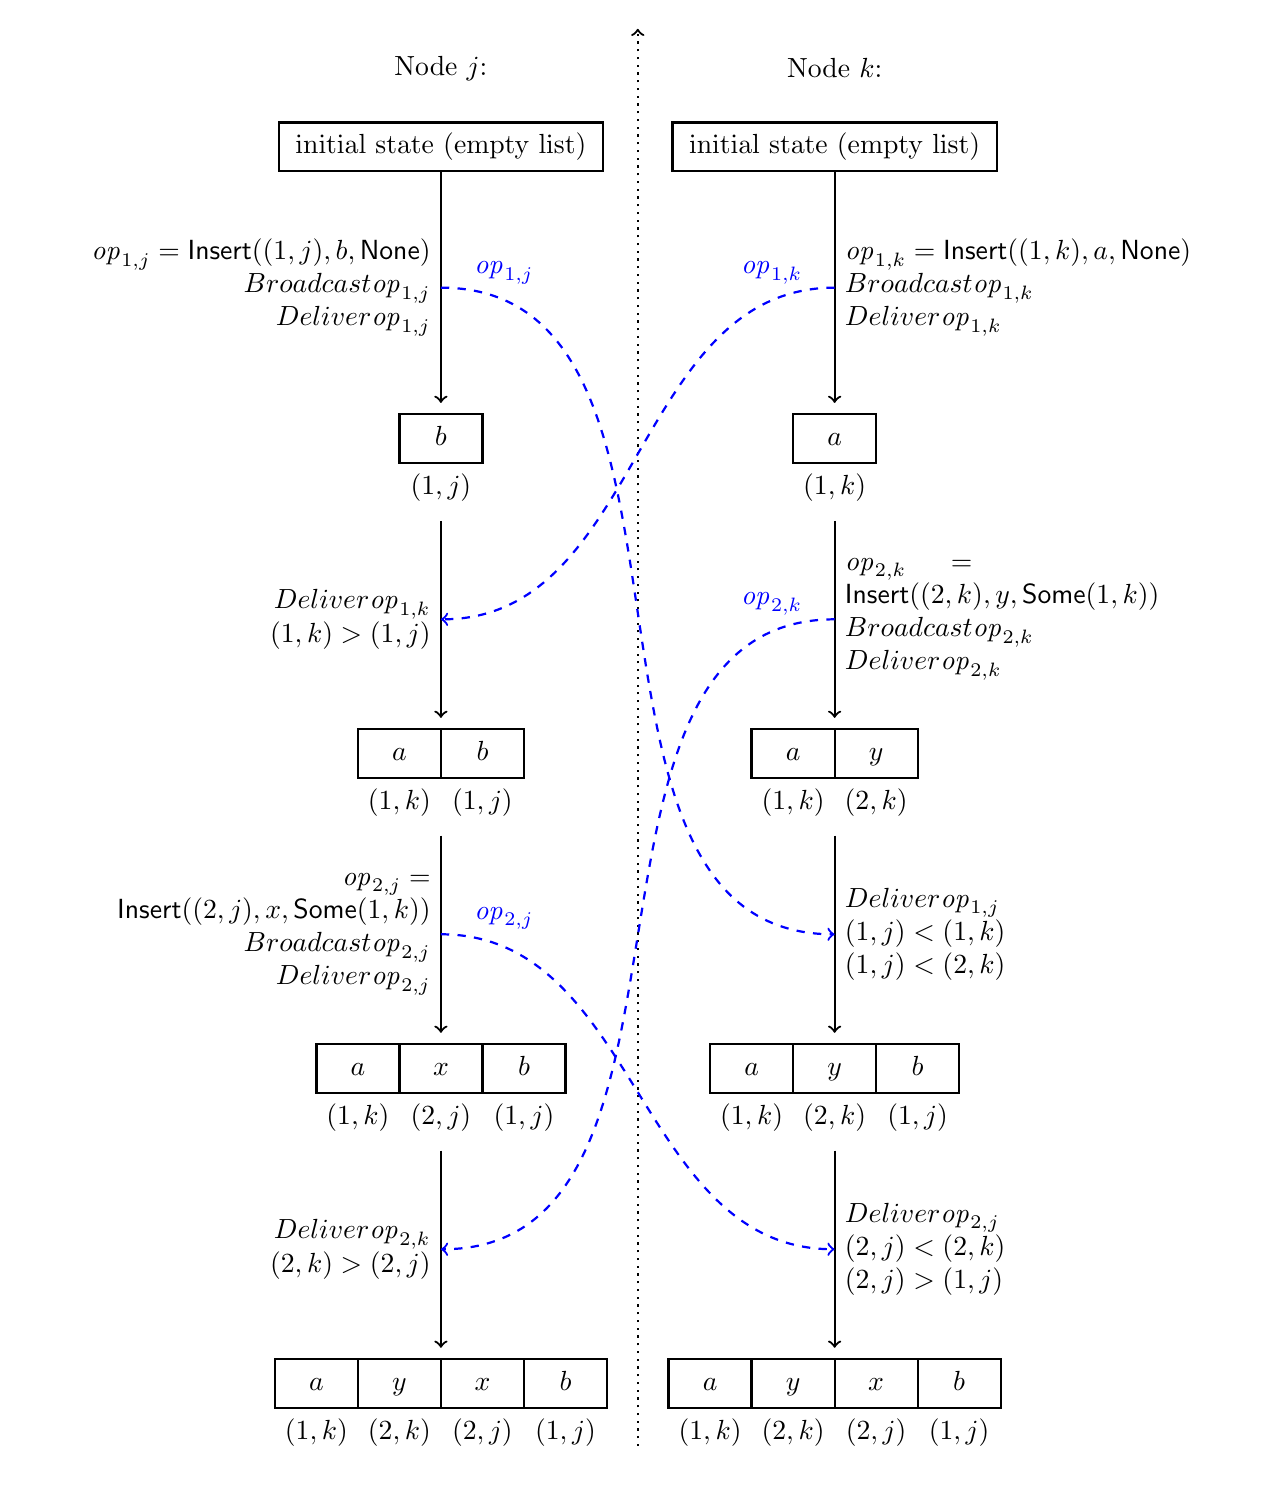
\begin{tikzpicture}[auto,scale=1.0]
\onehalfspacing
\path [draw,dotted] (2.5,-0.5) -- (2.5,17.5);

\tikzstyle{initstate}=[rectangle,draw,inner xsep=6pt,text height=8pt,text depth=3pt]
\tikzstyle{state}=[matrix,column sep={30pt,between origins}]
\tikzstyle{val}=[draw,anchor=base,minimum width=30pt,text height=8pt,text depth=3pt]
\tikzstyle{oid}=[anchor=base]
\tikzstyle{leftevent}=[left,text width=5cm,text ragged left,midway]
\tikzstyle{rightevent}=[right,text width=5cm,text ragged,midway]
\tikzstyle{every path}=[thick,->]

\node (leftR) at (0,17) {Node $j$:};
\node (left1) at (0,16) [initstate] {initial state (empty list)};
\node (left2) at (0,12) [state] {
    \node [val] {$b$};     \\
    \node [oid] {$(1,j)$}; \\
};
\node (left3) at (0,8) [state] {
    \node [val] {$a$};     & \node [val] {$b$};     \\
    \node [oid] {$(1,k)$}; & \node [oid] {$(1,j)$}; \\
};
\node (left4) at (0,4) [state] {
    \node [val] {$a$};     & \node [val] {$x$};     & \node [val] {$b$};     \\
    \node [oid] {$(1,k)$}; & \node [oid] {$(2,j)$}; & \node [oid] {$(1,j)$}; \\
};
\node (left5) at (0,0) [state] {
    \node [val] {$a$};     & \node [val] {$y$};     & \node [val] {$x$};     & \node [val] {$b$};     \\
    \node [oid] {$(1,k)$}; & \node [oid] {$(2,k)$}; & \node [oid] {$(2,j)$}; & \node [oid] {$(1,j)$}; \\
};

\draw (left1) -- (left2) node (send1j) [leftevent] {
    \hfill $\mathit{op}_{1,j} = \mathsf{Insert}((1, j), b, \mathsf{None})$ \\
    \hfill $\text{Broadcast } \mathit{op}_{1,j}$ \\
    \hfill $\text{Deliver } \mathit{op}_{1,j}$ \\
};
\draw (left2) -- (left3) node (recv1k) [leftevent] {
    \hfill $\text{Deliver } \mathit{op}_{1,k}$ \\
    \hfill $(1,k) > (1,j)$ \\
};
\draw (left3) -- (left4) node (send2j) [leftevent] {
    \hfill $\mathit{op}_{2,j} = \mathsf{Insert}((2, j), x, \mathsf{Some}(1,k))$ \\
    \hfill $\text{Broadcast } \mathit{op}_{2,j}$ \\
    \hfill $\text{Deliver } \mathit{op}_{2,j}$ \\
};
\draw (left4) -- (left5) node (recv2k) [leftevent] {
    \hfill $\text{Deliver } \mathit{op}_{2,k}$ \\
    \hfill $(2,k) > (2,j)$ \\
};

\node (rightR) at (5,17) {Node $k$:};
\node (right1) at (5,16) [initstate] {initial state (empty list)};
\node (right2) at (5,12) [state] {
    \node [val] {$a$};     \\
    \node [oid] {$(1,k)$}; \\
};
\node (right3) at (5,8) [state] {
    \node [val] {$a$};     & \node [val] {$y$};     \\
    \node [oid] {$(1,k)$}; & \node [oid] {$(2,k)$}; \\
};
\node (right4) at (5,4) [state] {
    \node [val] {$a$};     & \node [val] {$y$};     & \node [val] {$b$};     \\
    \node [oid] {$(1,k)$}; & \node [oid] {$(2,k)$}; & \node [oid] {$(1,j)$}; \\
};
\node (right5) at (5,0) [state] {
    \node [val] {$a$};     & \node [val] {$y$};     & \node [val] {$x$};     & \node [val] {$b$};     \\
    \node [oid] {$(1,k)$}; & \node [oid] {$(2,k)$}; & \node [oid] {$(2,j)$}; & \node [oid] {$(1,j)$}; \\
};

\draw (right1) -- (right2) node (send1k) [rightevent] {
    $\mathit{op}_{1,k} = \mathsf{Insert}((1, k), a, \mathsf{None})$ \\
    $\text{Broadcast } \mathit{op}_{1,k}$ \\
    $\text{Deliver } \mathit{op}_{1,k}$ \\
};
\draw (right2) -- (right3) node (send2k) [rightevent] {
    $\mathit{op}_{2,k} = \mathsf{Insert}((2, k), y, \mathsf{Some}(1, k))$ \\
    $\text{Broadcast } \mathit{op}_{2,k}$ \\
    $\text{Deliver } \mathit{op}_{2,k}$ \\
};
\draw (right3) -- (right4) node (recv1j) [rightevent] {
    $\text{Deliver } \mathit{op}_{1,j}$ \\
    $(1,j) < (1,k)$ \\
    $(1,j) < (2,k)$ \\
};
\draw (right4) -- (right5) node (recv2j) [rightevent] {
    $\text{Deliver } \mathit{op}_{2,j}$ \\
    $(2,j) < (2,k)$ \\
    $(2,j) > (1,j)$ \\
};

\begin{scope}[dashed,blue]
    \tikzstyle{every node}=[text centered]
    \draw (send1j.east) to [out=0,in=180] (recv1j.west);
    \draw (send2j.east) to [out=0,in=180] (recv2j.west);
    \draw (send1k.west) to [out=180,in=0] (recv1k.east);
    \draw (send2k.west) to [out=180,in=0] (recv2k.east);
    \node at (0.8,14.4) {$\mathit{op}_{1,j}$};
    \node at (0.8, 6.2) {$\mathit{op}_{2,j}$};
    \node at (4.2,14.4) {$\mathit{op}_{1,k}$};
    \node at (4.2,10.2) {$\mathit{op}_{2,k}$};
\end{scope}
\end{tikzpicture}
